%Thedore Ian Martiny
%Summer 2017 Homework 5

\documentclass[addpoints]{exam}
\newcommand{\naturals}{\mathbb{N}}
\newcommand{\reals}{\mathbb{R}}
\newcommand{\integers}{\mathbb{Z}}
\newcommand{\rationals}{\mathbb{Q}}
\renewcommand{\baselinestretch}{1.5}
%\setlength{\textwidth}{16cm}
\usepackage{amsfonts}
\usepackage{amsmath}
\usepackage{amsthm}
\usepackage{amssymb}
\usepackage{color}
\usepackage{colortbl}
\usepackage{fullpage}
\usepackage{graphicx}
\usepackage[utf8]{inputenc}
\usepackage{listings}
\usepackage{multicol}
\usepackage{setspace}
\usepackage{wasysym}
\usepackage{xcolor}
 
\definecolor{codegreen}{rgb}{0,0.6,0}
\definecolor{codegray}{rgb}{0.5,0.5,0.5}
\definecolor{codepurple}{rgb}{0.58,0,0.82}
\definecolor{backcolour}{rgb}{0.95,0.95,0.92}
\definecolor{Gray}{gray}{0.85}
 
\lstdefinestyle{mystyle}{
    backgroundcolor=\color{backcolour},   
    commentstyle=\color{codegreen},
    keywordstyle=\color{magenta},
    numberstyle=\tiny\color{codegray},
    stringstyle=\color{codepurple},
    basicstyle=\footnotesize,
    breakatwhitespace=false,         
    breaklines=true,                 
    captionpos=b,                    
    keepspaces=true,                 
    numbers=left,                    
    numbersep=5pt,                  
    showspaces=false,                
    showstringspaces=false,
    showtabs=false,                  
    tabsize=2
}
\newcolumntype{a}{>{\columncolor{Gray}}c} 
\lstset{style=mystyle}
\begin{document}
\singlespacing

\begin{center}
  {\large\textbf{CSCI 2824 - Discrete Structures}}

  {\large\textbf{Homework 5}}
\end{center}

You MUST show your work. If you only present answers you will receive minimal 
credit. This homework is worth \numpoints pts.

This homework contains some problems which will require you to show work in the
form of a program. You may use any language you wish. As usual using a language
other than Python and C/C++ will result in extra credit.

The homework 5 submission on Moodle will allow 3 file submissions: one for .pdf,
one for .tex, one for tarball with code. The tarball you submit must contain
separate files for the code for each problem, that is not one file solving both
problems, but each problem solved separately. Additionally you need to include a
Makefile. It should contain at least two rules, one called \texttt{all:} which
will compile your file if necessary (or print a message saying you don't need
to compile your code) and one called \texttt{run:} which will run both of your
solutions back-to-back. This way it does not matter what you call your files, or
if you use third-party libraries (only use third-party libraries for Big
Integers, if your language does not support them) that need command line
arguments the grader does not need to know, he can simply type \texttt{\$ make} 
and then \texttt{\$ make run} and have your code compile/print a message and
execute.

\textbf{Due: Wednesday July 19}

\begin{questions}
  %%% Question 1
  \question[12] Find the prime factorizations of the following numbers:

  \begin{parts}
    \part 209
    \begin{solution}
      $209 = 11 \cdot 19$
    \end{solution}

    \part 637
    \begin{solution}
        $637 = 7^2 \cdot 13$
    \end{solution}

    \part 1050703
    \begin{solution}
      $1050703 = 101^2 \cdot 103$
    \end{solution}

    \part $11!$
    \begin{solution}
      \begin{align*}
        11! &= 11\cdot 10 \cdot 9 \cdot 8\cdots 2\cdot 1\\
        &= 11\cdot (5\cdot 2)\cdot (3\cdot 3)\cdot (2\cdot 2\cdot 2\cdot) \cdots
            2\cdot 1\\
        &= 11\cdot 7\cdot 5^2 \cdot 3^4 \cdot 2^8
      \end{align*}
    \end{solution}
  \end{parts}

  %%% Question 2
  \question[15] Find the greatest common divisor between the following pairs of
  numbers:

  \begin{parts}
    \part $13, 13^2$
    \begin{solution}
        13, they are given in their prime factorization, and the greatest common
        divisor between both is 13.
    \end{solution}

    \part $3^2\cdot 7^3\cdot 11, 3\cdot 7^5\cdot 11$
    \begin{solution}
        $3\cdot 7^3 \cdot 11$. Again they are given in their prime
        factorization, so we can simply pick off the highest power of each prime
        that is in both.
    \end{solution}

    \part $220, 1400$
    \begin{solution}
        Here we use the Euclidean Algorithm:
        \begin{align*}
            1400 &= 6\cdot 220 + 80\\
            220 &= 2\cdot 80 + 60\\
            80 &= 1\cdot 60 + 20\\
            60 &= 3\cdot 20 + 0
        \end{align*}
        Thus $\gcd(220,1400) = 20$
    \end{solution}
  \end{parts}

  %%% Question 3
  \question[4] The Euler $\phi$-function (or totient function) is a function
    from $\naturals\to\naturals$ which returns the number of positive integers
    less than or equal to $n$ which are relatively prime to $n$. E.g. $\phi(6) =
    2$ since only $1,5$ are relatively prime to 6 between 1 and 6. $\phi(8) = 4$
    because $1, 3,5,7$ are the only values which are relatively prime between 1
    and 8.

  \begin{parts}
    \part Find $\phi(10)$
    \begin{solution}
        $\phi(10) = 3$ since only $3, 7, 9$ are relatively prime to 10 between 1
        and 10.
    \end{solution}

    \part Prove that $n$ is prime if and only if $\phi(n) = n-1$.
    \begin{solution}
        $(\Leftarrow)$ If $\phi(n) = n-1$ that means that every number between 1
        and $n$ is relatively prime to $n$ (excepting $n$ itself), thus $n$ has
        no prime factors smaller than it, it must be prime.

        $(\Rightarrow)$ If $n$ is prime then it has no prime factors smaller than
        it, meaning that $\gcd(n,i) = 1$ for all $i$ less than $n$. However
        $\gcd(n,n)= n$ so $\phi(n) = n-1$.
        \qed
    \end{solution}
  \end{parts}

  %%% Question 4
  \question[6] Solve the following congruences:
  \begin{parts}
    \part $19x \equiv 4 \mod 141$
    \begin{solution}
        We find the inverse of 19 modulo 141. First the Euclidean Algorithm:
        \begin{align*}
            141 &= 7\cdot 19 + 8\\
            19 &= 2\cdot 8 + 3\\
            8 &= 2\cdot 3 + 2\\
            3 &= 1\cdot 2 + 1
        \end{align*}
        Now we substitute backwards to solve for 1 (Extended Euclidean
        Algorithm):
        \begin{align*}
            1 &= 3 - 1\cdot 2\\
            &= 3 - 1\cdot (8 - 2\cdot 3)\\
            &= 3\cdot 3 - 1\cdot 8\\
            &= 3\cdot (19 - 2\cdot 8) - 1\cdot 8\\
            &= 3\cdot 19 - 7\cdot 8\\
            &= 3\cdot 19 - 7\cdot (141 - 7\cdot 19)\\
            &= 52\cdot 19 - 7\cdot 141
        \end{align*}
        Thus the $19^{-1}\mod 141 \equiv 52$.

        Now we can multiply both sides or our equation above by 52 to solve for
        $x$:
        \[
            x= 260 \equiv 119\mod 141
        \]
    \end{solution}

    \part $34x \equiv 77 \mod 89$
    \begin{solution}
        We find the inverse of 34 modulo 89. First the Euclidean Algorithm:
        \begin{align*}
            89 &= 2\cdot 34 + 21\\
            34 &= 1\cdot 21 + 13\\
            21 &= 1\cdot 13 + 8\\
            13 &= 1\cdot 8 + 5\\
            8 &= 1\cdot 5 + 3\\
            5 &= 1\cdot 3 + 2\\
            3 &= 1\cdot 2 + 1
        \end{align*}
        Now we substitute backwards to solve for 1 (Extended Euclidean
        Algorithm):
        \begin{align*}
            1 &= 3 - 1\cdot 2\\
            &= 3 - 1\cdot (5 - 1\cdot 3)\\
            &= 2\cdot 3 - 1\cdot 5\\
            &= 2\cdot (8 - 1\cdot 5) - 1\cdot 5\\
            &= 2\cdot 8 - 3\cdot 5\\
            &= 2\cdot 8 - 3\cdot (13 - 1\cdot 8)\\
            &= 5\cdot 8 - 3\cdot 13\\
            &= 5\cdot (21 - 1\cdot 13) - 3\cdot 13\\
            &= 5\cdot 21 - 8\cdot 13\\
            &= 5\cdot 21 - 8\cdot (34 - 1\cdot 21)\\
            &= 13\cdot 21 - 8\cdot 34\\
            &= 13\cdot (89 - 2\cdot 34) - 8\cdot 34\\
            &= 13\cdot 89 - 34\cdot 34
        \end{align*}
        Thus the $34^{-1}\mod 89 \equiv 34$.

        Now we can multiply both sides or our equation above by 52 to solve for
        $x$:
        \[
            x= 2618 \equiv 37\mod 89 
        \]
    \end{solution}
  \end{parts}

  %%% Question 5
  \question[8] Solve the following systems for a single $x$ (per part).
  \begin{parts}
    \part $x\equiv 2\mod 3$, $x\equiv 1\mod 4$, $x\equiv 3\mod 5$
    \begin{solution}
      Choose
      \[
        x = 2\cdot 4\cdot 5\cdot 2  + 1 \cdot 3\cdot 5\cdot 3 + 3\cdot 3\cdot
        4\cdot 3
      \]
      This yields $x = 233$ the unique solution modulo the product of individual
      moduli is: $x\equiv 53 \mod 60$.
    \end{solution}

    \part $x\equiv 1\mod 2$, $x\equiv 2\mod 3$, $x\equiv 3\mod 5$, $x\equiv
    4\mod 11$.
    \begin{solution}
      Choose
      \[
        x = 1\cdot 3\cdot 5\cdot 11\cdot 1 + 2\cdot 5\cdot 11\cdot 1 + 3\cdot
        2\cdot 11\cdot 3 + 4\cdot 3\cdot 5\cdot 3
      \]
      This yields $x = 653$, the unique solution modulo the product of
      individual moduli is $x \equiv 323 \mod 330$.
    \end{solution}
  \end{parts}
  
  %%% Question 6
  \question[10] Compute the following numbers:
  \begin{parts}
    \part $11^{644} \mod 645$
    \begin{solution}
        First we write $644$ in binary:
        \[
            644 = 512 + 128 +  4
        \]
        So:
        \[
            11^{644} \mod 645 = 11^{512}11^{128}11^4\mod 645
        \]
        Then we compute:
        \begin{align*}
            11^1 &= 11 \equiv 11\mod 645\\
            11^2 &= 121 \equiv 121\mod 645\\
            11^4 &= 14641 \equiv 451 \mod 645\\
            11^8 &= 203401 \equiv 226 \mod 645\\
            11^{16} &= 51076 \equiv 121 \mod 645\\
            11^{32} &= 14641 \equiv 451 \mod 645\\
            11^{64} &= 203401 \equiv 226 \mod 645\\
            11^{128} &= 51076 \equiv 121 \mod 645\\
            11^{256} &= 14641 \equiv 451 \mod 645\\
            11^{512} &= 203401 \equiv 226 \mod 645\\
        \end{align*}
        Thus
        \begin{align*}
            11^{644} \mod 645 &= 11^{512}11^{128}11^4\mod 645\\
            &= (226)\cdot(121)\cdot(451)\mod 645\\
            &= 12333046 \mod 645\\
            &\equiv 1
        \end{align*}
    \end{solution}

    \part $12^{2003} \mod 2037$
    \begin{solution}
        First we write $2003$ in binary:
        \[
            2003 = 1024 + 512 + 256 + 128 + 64 + 16 + 2 + 1
        \]
        So:
        \[
            12^{2003} \mod 2037 = 12^{1024}12^{512}12^{256}12^{128}12^
            {64}12^{16}12^212^1\mod 2037
        \]
        Then we compute:
        \begin{align*}
            12^1 &= 12 \equiv 12\mod 2037\\
            12^2 &= 144 \equiv 144\mod 2037\\
            12^4 &= 20736 \equiv 366 \mod 2037\\
            12^8 &= 133956 \equiv 1551  \mod 2037\\
            12^{16} &= 2405601 \equiv 1941 \mod 2037\\
            12^{32} &= 3767481 \equiv 1068 \mod 2037\\
            12^{64} &= 1140624 \equiv 1941 \mod 2037\\
            12^{128} &= 3767481 \equiv 1068 \mod 2037\\
            12^{256} &= 1140624 \equiv 1941 \mod 2037\\
            12^{512} &= 3767481 \equiv 1068 \mod 2037\\
            12^{1024} &= 1140624 \equiv 1941 \mod 2037
        \end{align*}
        Thus
        \begin{align*}
            12^{2003} \mod 2037 &= 12^{1024} 12^{512} 12^{256} 12^{128} 12^{64} 
                12^{16} 12^2 12^1\mod 2037\\
            &= (1941)\cdot(1068)\cdot(1941)\cdot(1068)\cdot(1941)\cdot
                (1941)\cdot(144)\cdot(12)\mod 2037\\
            &= 2072988 \cdot 2072988 \cdot 3767481 \cdot 1728\mod 2037\\
            &\equiv 1359 \cdot 1359 \cdot 1068 \cdot 1728 \mod 2037\\
            &= 1846881 \cdot 1845504 \mod 2037\\
            &\equiv 1359 \cdot 2019 \mod 2037\\
            &= 2743821 \mod 2037\\
            &\equiv 2019
        \end{align*}
    \end{solution}
  \end{parts}

  %%% Question 7
  \question[10] This is a programming problem, from Project Euler. The prime
  factors of 13195 are 5, 7, 13 and 29. What is the largest prime factor of the
  number 600851475143? 

  You may use any programming language to answer this  (though if you use a C
  variant you will probably need a third party library to represent that large a
  number). In your .pdf write up you should place the answer with an explanation
  of how you got it. You should also submit your code on Moodle (along with a
  Makefile for any compilation).
  \begin{solution}
    The solution is 6857.
  \end{solution}

  %%% Question 8
  \question[10] This is a programming problem, from Project Euler. By listing
  the first six prime numbers: 2, 3, 5, 7, 11, and 13, we can see that the 6th
  prime is 13. What is the 10,001st prime number?

  You may use any programming language to answer this  (though if you use a C
  variant you will probably need a third party library to represent that large a
  number). In your .pdf write up you should place the answer with an explanation
  of how you got it. You should also submit your code on Moodle (along with a
  Makefile for any compilation).
  \begin{solution}
    The solution is 104743.
  \end{solution}

  %%% Question 9
  \question[5] What sequence of pseudorandom numbers is generated using the pure
  multiplicative generator $x_{n+1} =3x_n \mod 11$ with seed $x_0 = 2$?
  \begin{solution}
    We can simply list the terms:
    \begin{align*}
        x_0 &= 2\\
        x_1 &= 3\cdot 2 = 6\\
        x_2 &= 3\cdot 6 = 18 \equiv 7\\
        x_3 &= 3\cdot 7 = 21 \equiv 10\\
        x_4 &= 3\cdot 10 = 30 \equiv 8\\
        x_5 &= 3\cdot 8 = 24 \equiv 2\\
        x_6 &= 3\cdot 2 = 6
    \end{align*}
    Since the next term is only dependent on the immediately previous term we
    can see our sequence will repeat after $x_6$. Thus the sequence is $2, 6,
    7, 10, 8$.
  \end{solution}

  %%% Question 10
  \question[5] Encrypt the message WATCH YOUR STEP using the encryption function
  $f(p) = 3p + 7 \mod 26$, by first converting the message into numbers as
  discussed in class.
  \begin{solution}
    WATCH YOUR STEP becomes: 2200190207 24142017 18190415.

    Multiplying each number by 3 and adding 7 modulo 26 yields:

    2107121302 01231506 09121900

    Which in letters is:
    VHMNC BXPG JMTA
  \end{solution}

  %% Question 11
  \question[5] Encrypt the message UPLOAD using the RSA encryption system as
  discussed in class. Use $n = 43\cdot 59$ and $e =13$. You may need to group
  letters together in different ways and pad with X's, if necessary. After
  encryption you may not be able to convert numbers back into letters, that is
  fine, however you should remember to pad the encrypted result back to a
  multiple of 2 digits. e.g. If the encryption of 12 is 5, you would print that
  as 05.
   \begin{solution}
        UPLOAD becomes: 201511140003

        $n = 2537$ thus we split UPLOAD into: 2015 1114 0003 each part is
        encrypted separately:
        \begin{align*}
            2015^{13} \mod 2537 \equiv 1628\\
            1114^{13} \mod 2537 \equiv 0763\\
            0003^{13} \mod 2537 \equiv 1087
        \end{align*}
        Thus the message we send is: 162807631087
   \end{solution}

   %%% Question 12
  \question[10] In class we discussed the Diffie-Hellman Key Exchange. The
  method discussed in class has a vulnerability. 

  Eve, an attacker, can alter messages that Alice and Bob send to each other
  without their knowing. To do this she intercepts (and makes some changes to) 
  the exchanges Alice and Bob make with each other. Discover this method and
  describe it to me.

  Hint: You should be attacking the key-exchange. Find a method so that Alice
  and Eve have shared keys and Eve and Bob have shared keys (even though Alice
  thinks she is communicating with Bob and Bob thinks he is communicating with
  Alice). And remember that Eve can intercept any message Alice sends to
  Bob and vice versa. This means that she can stop the message from reaching its
  destination and send another in its place.
  \begin{solution}
    This is called a Man-in-the-Middle attack. It works as follows:

    Since Eve gets to look at every message (including the key exchange steps)
    she can simply play both sides of the conversation. That is she can work the
    key exchange protocol with Alice to find her key while simultaneously doing
    a key exchange with Bob. To do so Eve will need to generate $e, E$ where
    $e,E$ are her exponents, that is $eE\equiv 1\mod (p-1)$ (just
    as Alice has $a,A$ and Bob has $b,B$).

    Then our communication will look as follows:
    \begin{center}
      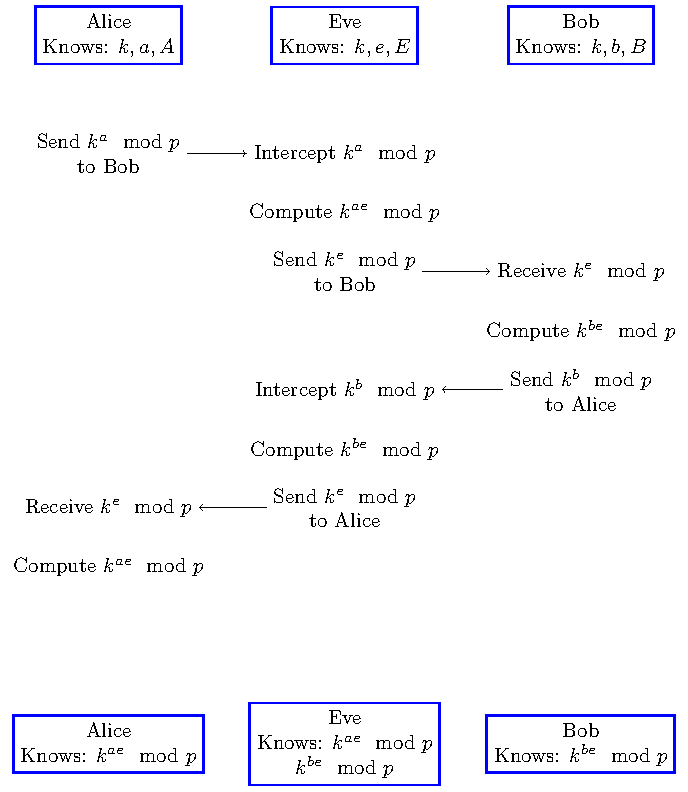
\includegraphics{AliceEveBob}
      \label{fig:MITM}
    \end{center}

    By communicating in this fashion Eve starts with no knowledge of Alice's key
    and acts as if both Alice and Bob are communicating directly with her and
    shares keys with them both.     

    After this communication Even can decrypt Alice's messages and determine
    what she wants to tell Bob and re-encrypt under their shared key to send to
    him.
  \end{solution}
\end{questions}
\end{document}
